\chapter{CLANN}

\section{Введение}
В данной работе представлена термодинамически корректная гиперупругая модель CLANN 
(Convex Laplace Artificial Neural Network),
основанная на выпуклой нейросети и логарифмической параметризации деформации - тензоре Лапласа. 
Модель обеспечивает физически корректное интерполирование и экстраполирование поля напряжений и объективное описание механического поведения материалов при больших деформациях,
что б проверено при помощи обучения модели на синтетических и натурных данных, и валидации получившейся модели на численном эксперименте.

\section{Кинематика }
\textbf{Основные соотношения}

Мы рассматриваем равновесие тонкой несжимаемой гиперупругой мембраны под определенными нагрузками.
Деформация мембраны характеризуется деформацией её срединной поверхности. 
Обозначим через \(\mathbf{X}\) и \(\mathbf{x}\) положения точек в исходной (недеформированной) \(\Omega_0\) и текущей (деформированной) \(\Omega_t\) конфигурациях 
срединной поверхности мембраны соответственно. 
Деформация определяется отображением \(\mathbf{x} = \mathbf{x}(\mathbf{X})\), 
поверхностный градиент деформации \(\vect F = \dfrac{\partial\mathbf{x}}{\partial\mathbf{X}}\),
а правый тензор Коши—Грина \(\vect C = \vect F^{\top} \vect F\). 
Для определения меры деформации мы используем тензор Лапласа \(\vect{\xi} = (\xi_1 , \xi_2 , \xi_3)\) основанный на QR-разложении \(\vect F_{2d}\) \cite{xi2023}.
В параметризации Холецкого \(\vect C = \vect U^{\top}\vect U\), где \(\vect U\) — верхнетреугольный тензор \cite{ddaniso2024}. 
В этом случае гиперупругий потенциал это функция от деформации Лапласа \(\psi = \psi(\vect{\xi})\).


\textbf{Мера деформации Лапласа}
В двумерном случае вводятся координаты
\begin{equation}
\xi_1 = \ln(u_{11}),\quad \xi_2 = \ln(u_{22}),\quad \xi_3 = \frac{u_{12}}{u_{11}},\quad u_{ij} \, \text{-- компоненты тензора} \, \vect U.
\end{equation}

% Данная параметризация улучшает обусловленность при больших деформациях и поддерживает выпуклое моделирование энергии в переменных \(\xi\).

\section{Напряжения и термодинамическая корректность}
\textbf{Гиперупругие напряжения} получаются дифференцированием энергии по мере деформации:
\begin{equation}
 \vect S = \frac{\partial\psi}{\partial\vect C} = \frac{\partial\psi}{\partial \xi}\,\frac{\partial \xi}{\partial \vect C},\qquad \vect r=\frac{\partial\psi}{\partial\xi}.
\label{eq:hyperelastic_stress}
\end{equation}
Такое построение гарантирует объективность и консервативность напряжений.

\textbf{Компоненты напряжений в двумерном случае} для выбранной параметризации в 2D будут следующими:
\begin{equation}
\begin{aligned}
  S_{11} &= e^{-2\xi_1}\big(r_1-2\xi_3 r_3\big) + e^{-2\xi_2} r_2\,\xi_3^2,\\
  S_{22} &= e^{-2\xi_2} r_2,\\
  S_{12} &= -e^{-2\xi_2} r_2\,\xi_3 + e^{-2\xi_1} r_3.
\end{aligned}
\end{equation}

\textbf{?Механические ограничения гиперупругости.}

\textbf{Положительность и рост энергии:}
\begin{equation}
 \psi(\xi) \ge 0\ \ \forall\,\xi\in\mathbb{R}^3,\qquad \psi(\xi) \to \infty\ \text{при}\ \lVert\xi\rVert\to\infty.
\end{equation}
Это обеспечивается \(\vect W_2\ge 0\), положительной активацией и выпуклостью.

\textbf{Симметрия и объективность:}
\begin{equation}
 S_{ij} = S_{ji},\qquad \psi = \psi(\vect C)\ \Rightarrow\ \text{инвариантность относительно поворотов}.
\end{equation}

% \textbf{?Консервативность напряжений:}
% \begin{equation}
%  \oint \vect S : d\vect C = 0.
% \end{equation}

\section{ICNN: архитектура и обучение}
\textbf{Строго выпуклая энергия}
Энергия деформации \(\psi(\xi)\) задаётся входной выпуклой нейросетью (ICNN):
\begin{equation}
 z=\frac{\operatorname{softplus}(\beta\,\vect W_1\xi)}{\beta},\qquad \psi=\vect W_2^{\top}z+b_2,\qquad \vect W_2\ge 0.
\end{equation}
Отсюда гессиан \(\vect H=\partial^2\psi/\partial\xi^2\) положительно определён.

\begin{figure}[htbp]
\centering
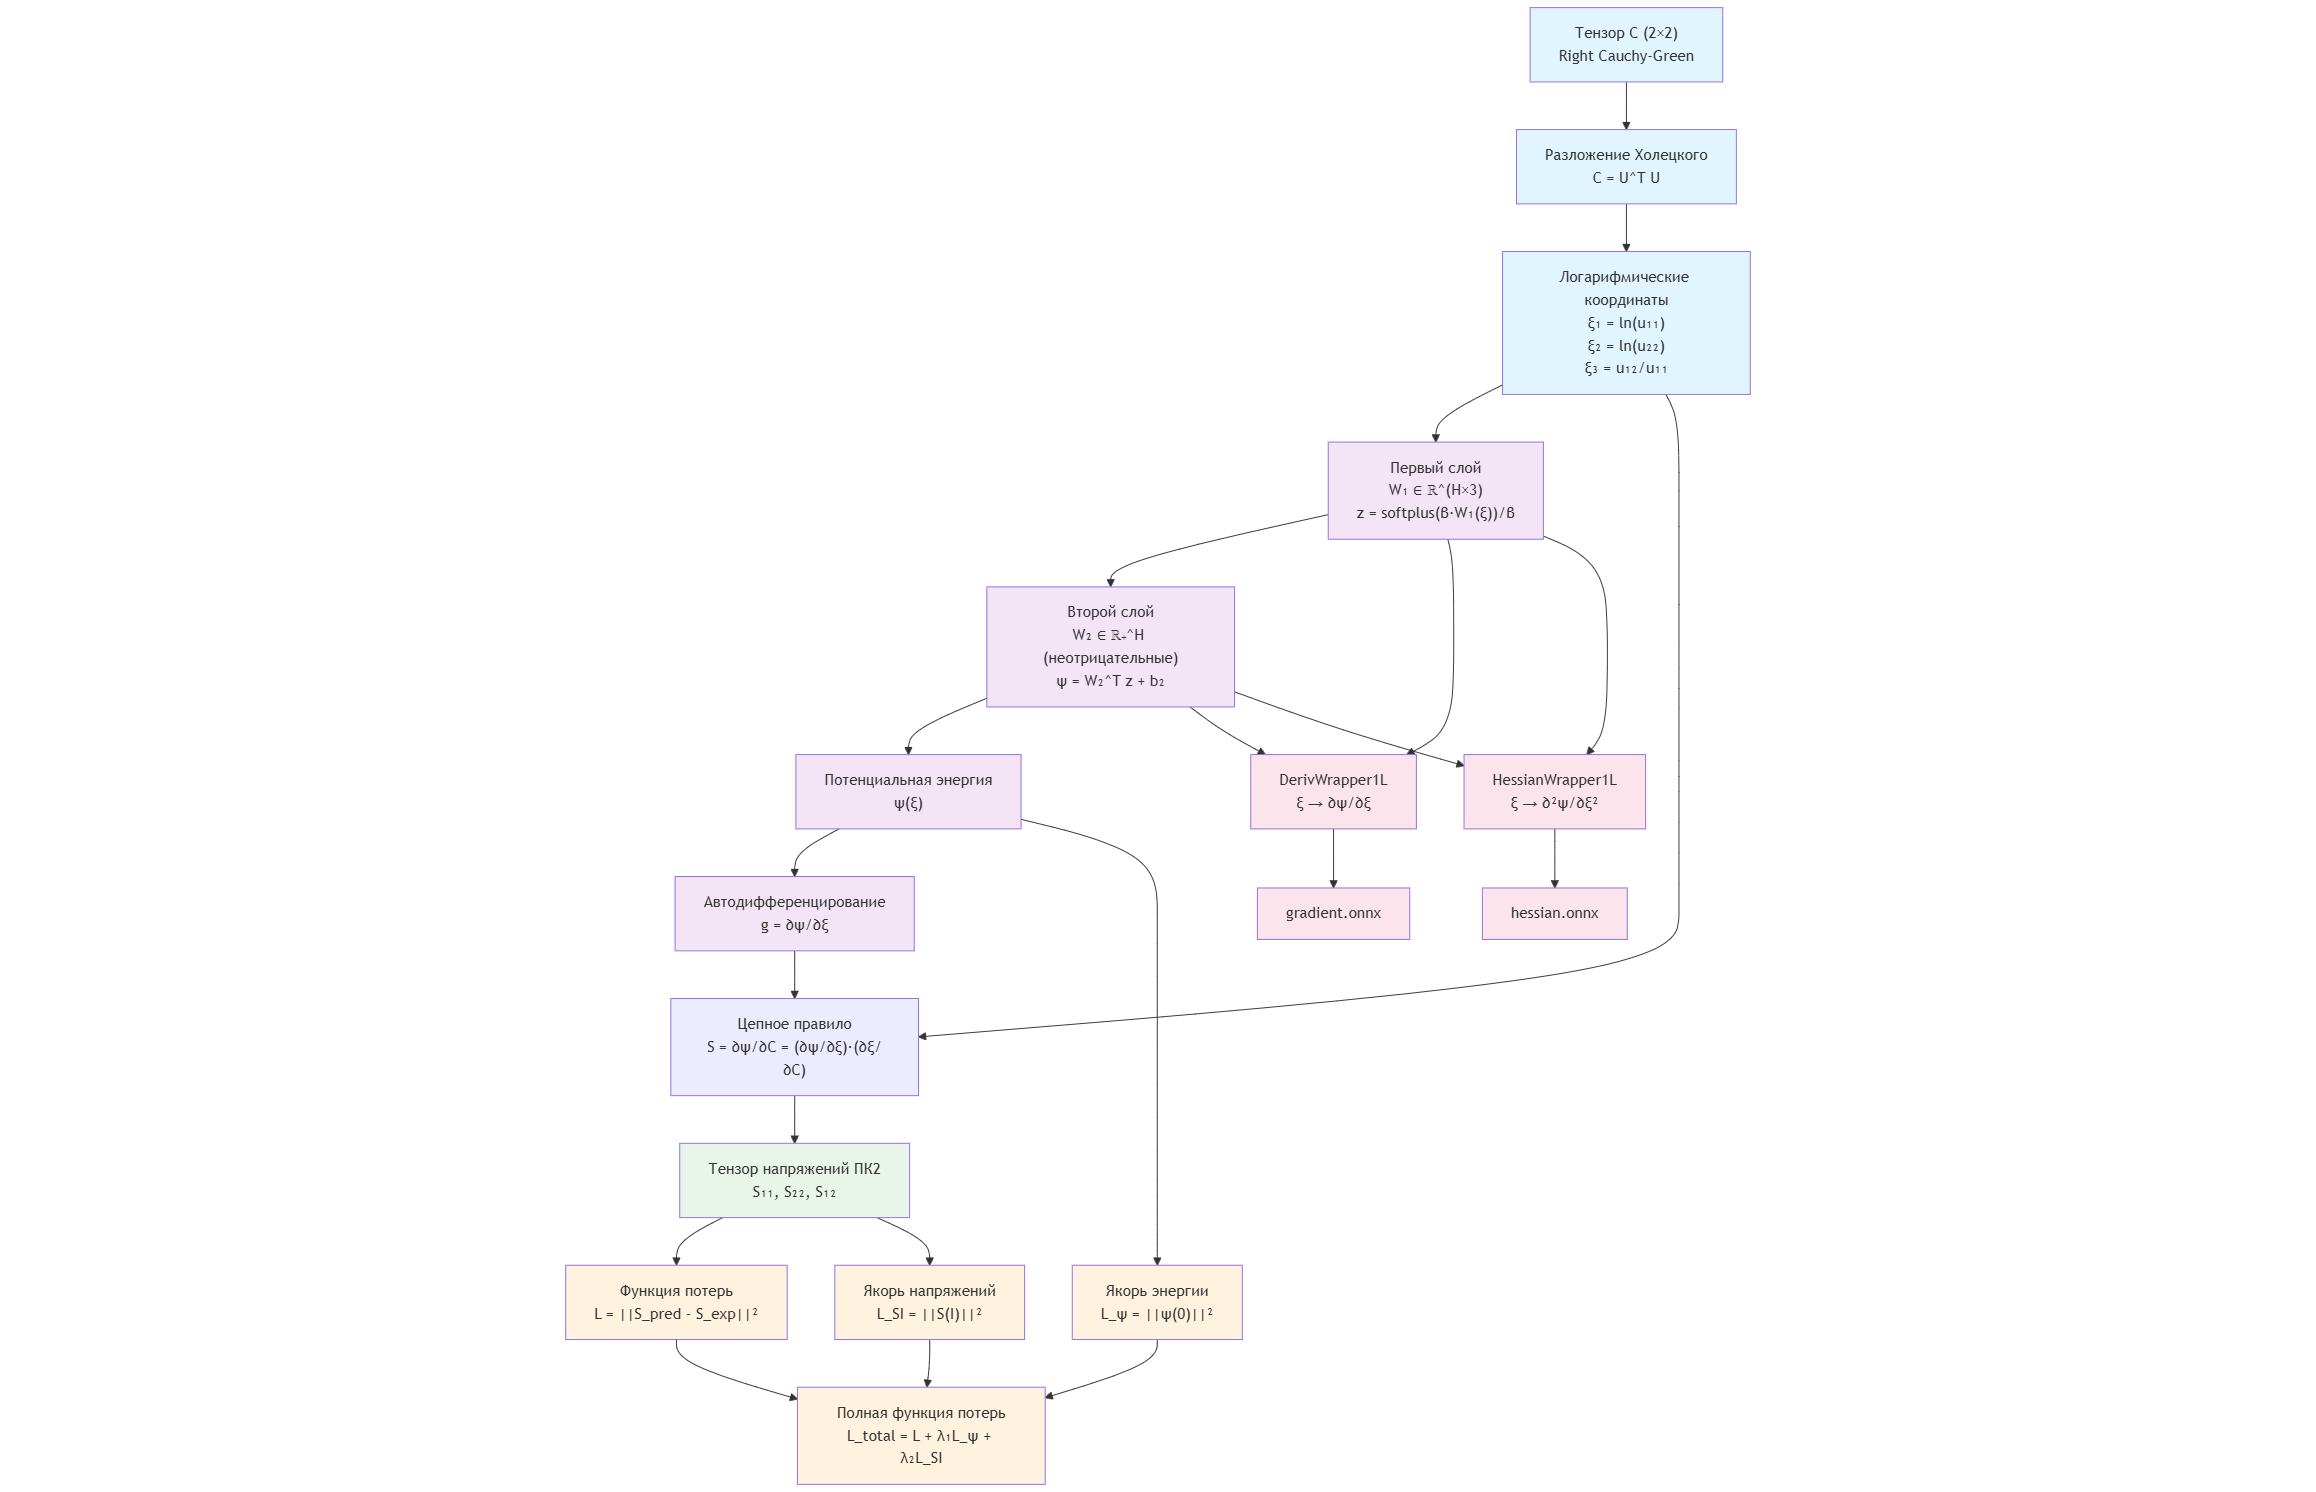
\includegraphics[width=1.3\textwidth]{img/clann_arc.png}
\caption{Схема вычислительного процесса CLANN: от входного тензора до функции потерь. Показаны этапы обработки входных данных, вычисления нейросетью, дифференцирования и формирования функции потерь.}
\label{fig:clann_architecture}
\end{figure}

\textbf{Аналитический градиент архитектуры ICNN}
Аналитическая форма градиента ICNN имеет вид
\begin{equation}
 \nabla_\xi \psi = W_1^T \left( w_2 \odot \sigma(\beta (W_1 \xi)) \right),
\end{equation}
где $\sigma(x) = \frac{1}{1 + e^{-x}}$ - сигмоида.

\textbf{Аналитический гессиан}
Аналитическая форма гессиана ICNN имеет вид
\begin{equation}
 H_{ij} = \sum_h \sigma'_h\,w_{2,h}\,W_{h,i}W_{h,j},\quad \sigma' = \beta\,\sigma(1-\sigma),\ \sigma=\operatorname{sigmoid}(\beta s),\ s=\vect W_1\xi+\vect b_1.
\end{equation}

\subsection{Функция потерь и обучение}
\subsubsection{Основная функция потерь}
\begin{equation}
 L = \frac{1}{N}\sum_{i=1}^N \lVert \vect S^{(i)}_{\text{pred}} - \vect S^{(i)}_{\text{exp}} \rVert^2.
\end{equation}

\subsubsection{Якорные слагаемые}
\begin{equation}
 L_{\text{SI}} = \lVert \vect S(\vect I)\rVert^2,\qquad L_{\psi}=\lVert\psi(0)\rVert^2.
\end{equation}
Полная функция потерь:
\begin{equation}
 L_{\text{total}} = L + \lambda_{\text{SI}} L_{\text{SI}} + \lambda_{\psi} L_{\psi}.
\end{equation}

Обучение прводилось на наборах данных с набором из 90 точек деформаций \(\mathbf{C}\) и напряжения \(\mathbf{S}\)
для двухосного растяжения тела с геометрией мальтийский крест. 
Гиперпараметры модели были следующие: learning rate = 0.001, batch size = 128, \(\lambda_{\text{SI}} = 0.1\), \(\lambda_{\psi} = 0.1\), количество нейронов на скрытом слое = 16.
Ошибка упала за менее чем 5000 эпох на 5 порядков.

\subsection{Интерполяция и экстраполяция кривых нагружения}
  вставить рисунок

\subsection{? Численные аспекты и интеграция в МКЭ}
\subsubsection{Разложение Холецкого}
\(\vect C = \vect U^{\top}\vect U\), \; \(\vect U=\operatorname{cholesky\_upper}(\vect C)\).

\subsubsection{Автоматическое дифференцирование и экспорт}
Используются автодифференцирование для \(\vect r=\partial\psi/\partial\xi\) и аналитические формулы для \(\vect S\) и гессиана; возможен экспорт вычислителей в онлайновые форматы.

\textbf{Физическая корректность и стабильность ICNN}

Архитектура ICNN обеспечивает несколько ключевых свойств, критически важных для физической корректности модели:

\textbf{Объективность}: Модель инвариантна относительно поворотов благодаря параметризации через инварианты деформации. Это гарантирует, что предсказания напряжений не зависят от выбора системы координат.

\textbf{Выпуклость энергии}: Строгая выпуклость \(\psi(\xi)\) обеспечивает единственность решения задачи минимизации энергии и положительную определённость касательной жёсткости. Это критически важно для стабильности численного решения в конечно-элементных расчётах.

\textbf{Положительность энергии}: Ограничение \(\vect W_2 \geq 0\) вместе с положительной активацией softplus гарантирует, что \(\psi(\xi) \geq 0\) для всех допустимых деформаций, что соответствует физическому принципу положительности энергии деформации.

\textbf{Стабильность численного решения}: Положительная определённость гессиана \(\vect H = \partial^2\psi/\partial\xi^2\) обеспечивает сходимость метода Ньютона при решении нелинейных уравнений равновесия. Это свойство особенно важно при больших деформациях, когда классические модели могут терять устойчивость.

\textbf{Регуляризация и обобщающая способность}: Выпуклая структура ICNN естественным образом предотвращает переобучение и обеспечивает плавную интерполяцию между точками обучения. Модель способна к экстраполяции за пределы диапазона обучающих данных благодаря физически обоснованной структуре энергии.

\textbf{Эффективность вычислений}: Аналитические выражения для градиента и гессиана позволяют избежать дорогостоящего численного дифференцирования, что критично для интеграции в конечно-элементные пакеты и реального времени расчётов.

\textbf{Термодинамическая корректность}: прямое вычисление напряжений из автоматического дифференцирования функции энергии по формуле \eqref{eq:hyperelastic_stress} гарантирует термодинамическую корректность.

\section{Численные эксперименты}

В первом эксперимнте CLANN был обучен на синтетических данных двухосного растяжения тела с геометрией мальтийский крест и потенциалом неогук 

\begin{table}[htbp]
\centering
\caption{Сводка проведенных экспериментов по обучению и валидации модели CLANN}
\label{tab:experiments_summary}
\begin{tabular}{|p{2.3cm}|p{2.2cm}|p{2.2cm}|p{1.3cm}|p{2.3cm}|p{1.5cm}|p{2.5cm}|}
\hline
\multicolumn{4}{|c|}{\textbf{Обучение}} & \multicolumn{3}{c|}{\textbf{Валидация}} \\
\hline
\textbf{Геометрия} & \textbf{Размер} & \textbf{Материал} & \textbf{Время} & \textbf{Геометрия} & \textbf{Время расчета} & \textbf{Количество элементов} \\
\hline
Мальтийский крест & 90 & Нео-Гук & -- & Гетерогенная круглая мембрана  & 329.816 сек & 4886 \\
\hline
Мальтийский крест & & & & Гомогенная круглая мембрана  & 329.816 сек & 4886  \\
\hline
Мальтийский крест & & & & Чистый сдвиг & -- сек & -- \\
\hline
\end{tabular}
\end{table}

\subsection{Сравнение с классическими моделями на синтетических данных}
Для оценки качества модели CLANN проведено сравнение с классической гиперупругой моделью Нео-Гука.
Для валидации модели CLANN на синтетических данных были проведены численные эксперименты с различными типами деформаций. 

\begin{figure}[htbp]
\centering
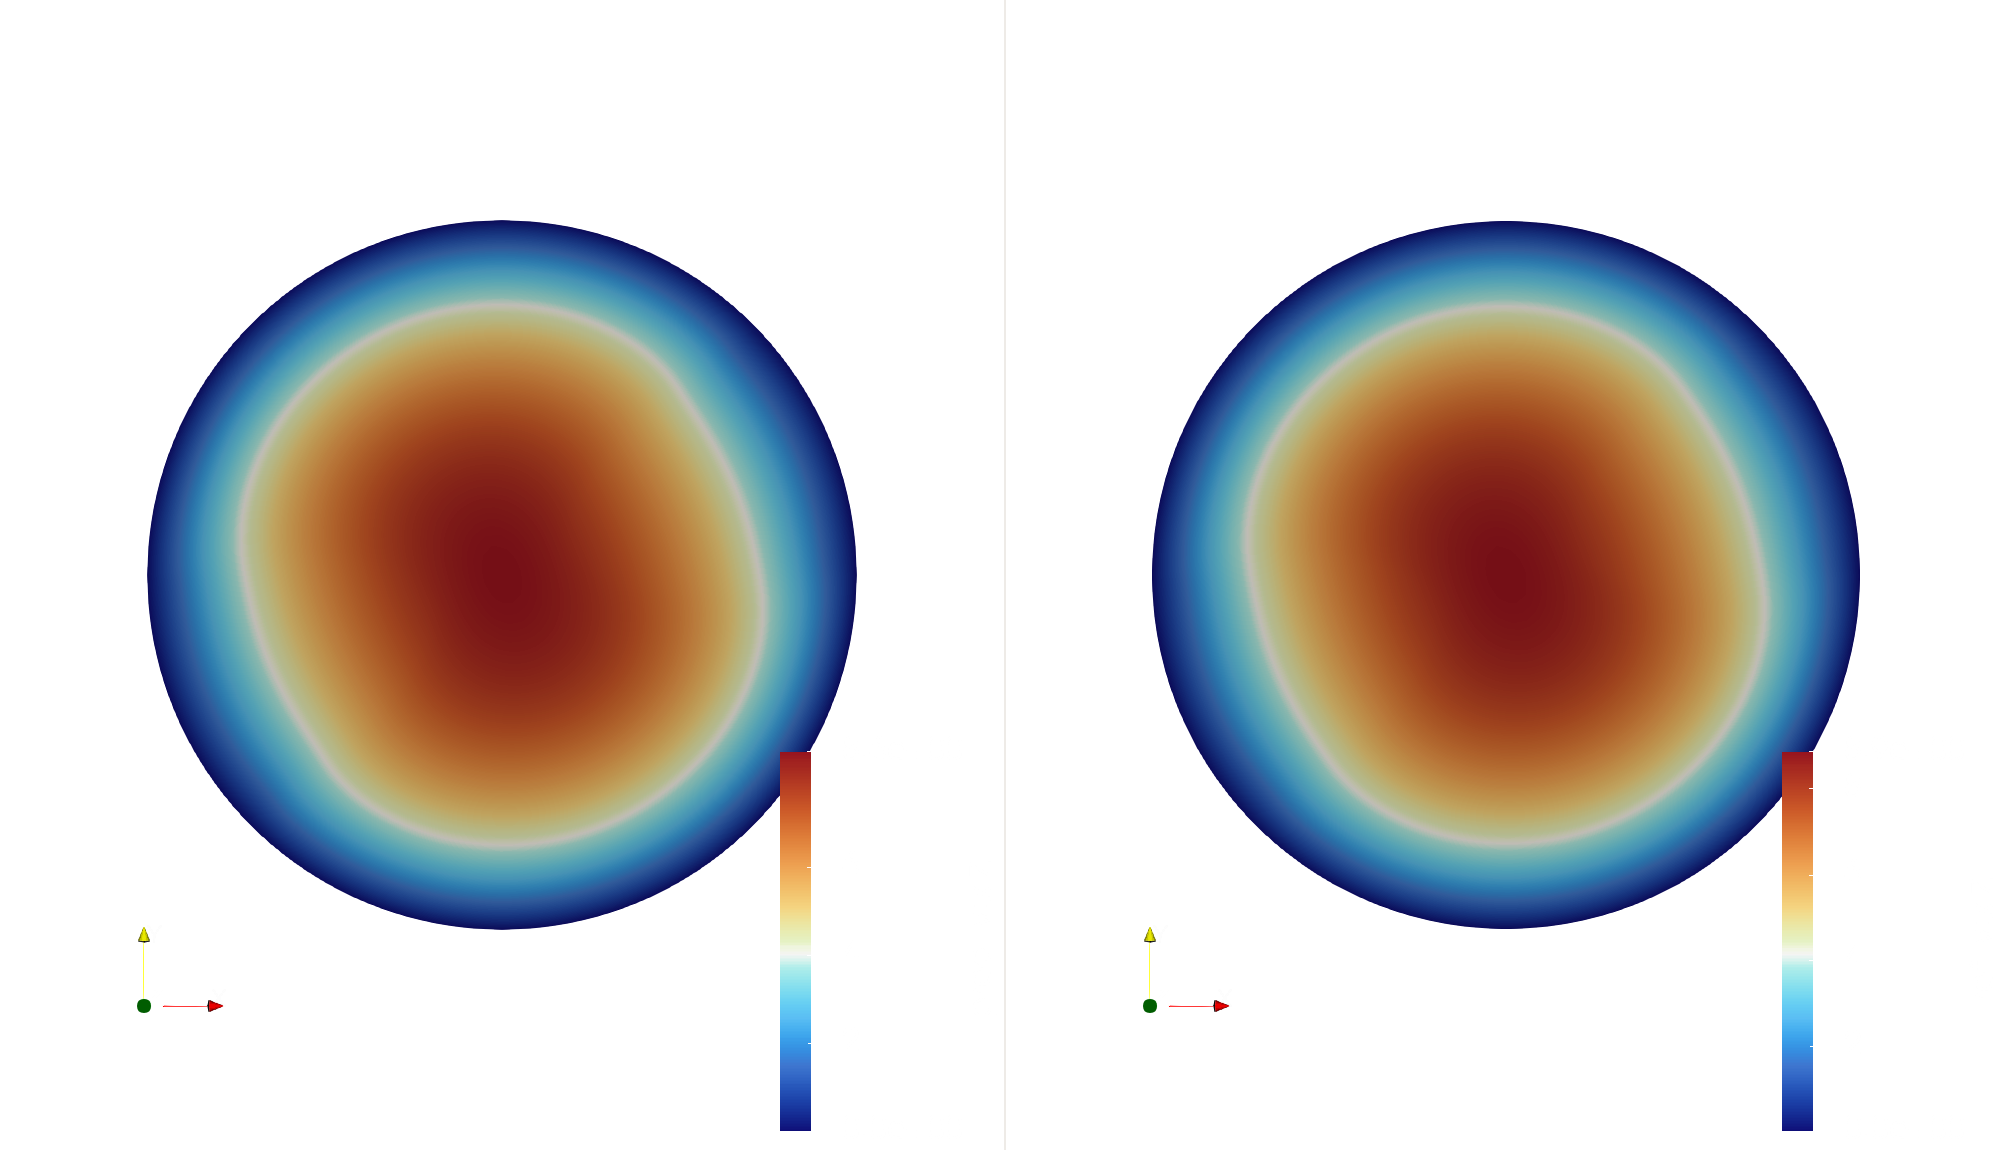
\includegraphics[width=0.8\textwidth]{img/bx_inf_u.png}
\caption{Результаты численного эксперимента: поле деформаций при различных типах нагружения. Показаны компоненты деформации $u_{11}$, $u_{22}$ и $u_{12}$ для различных конфигураций нагружения.}
\label{fig:numerical_deformations}
\end{figure}

\begin{figure}[htbp]
\centering
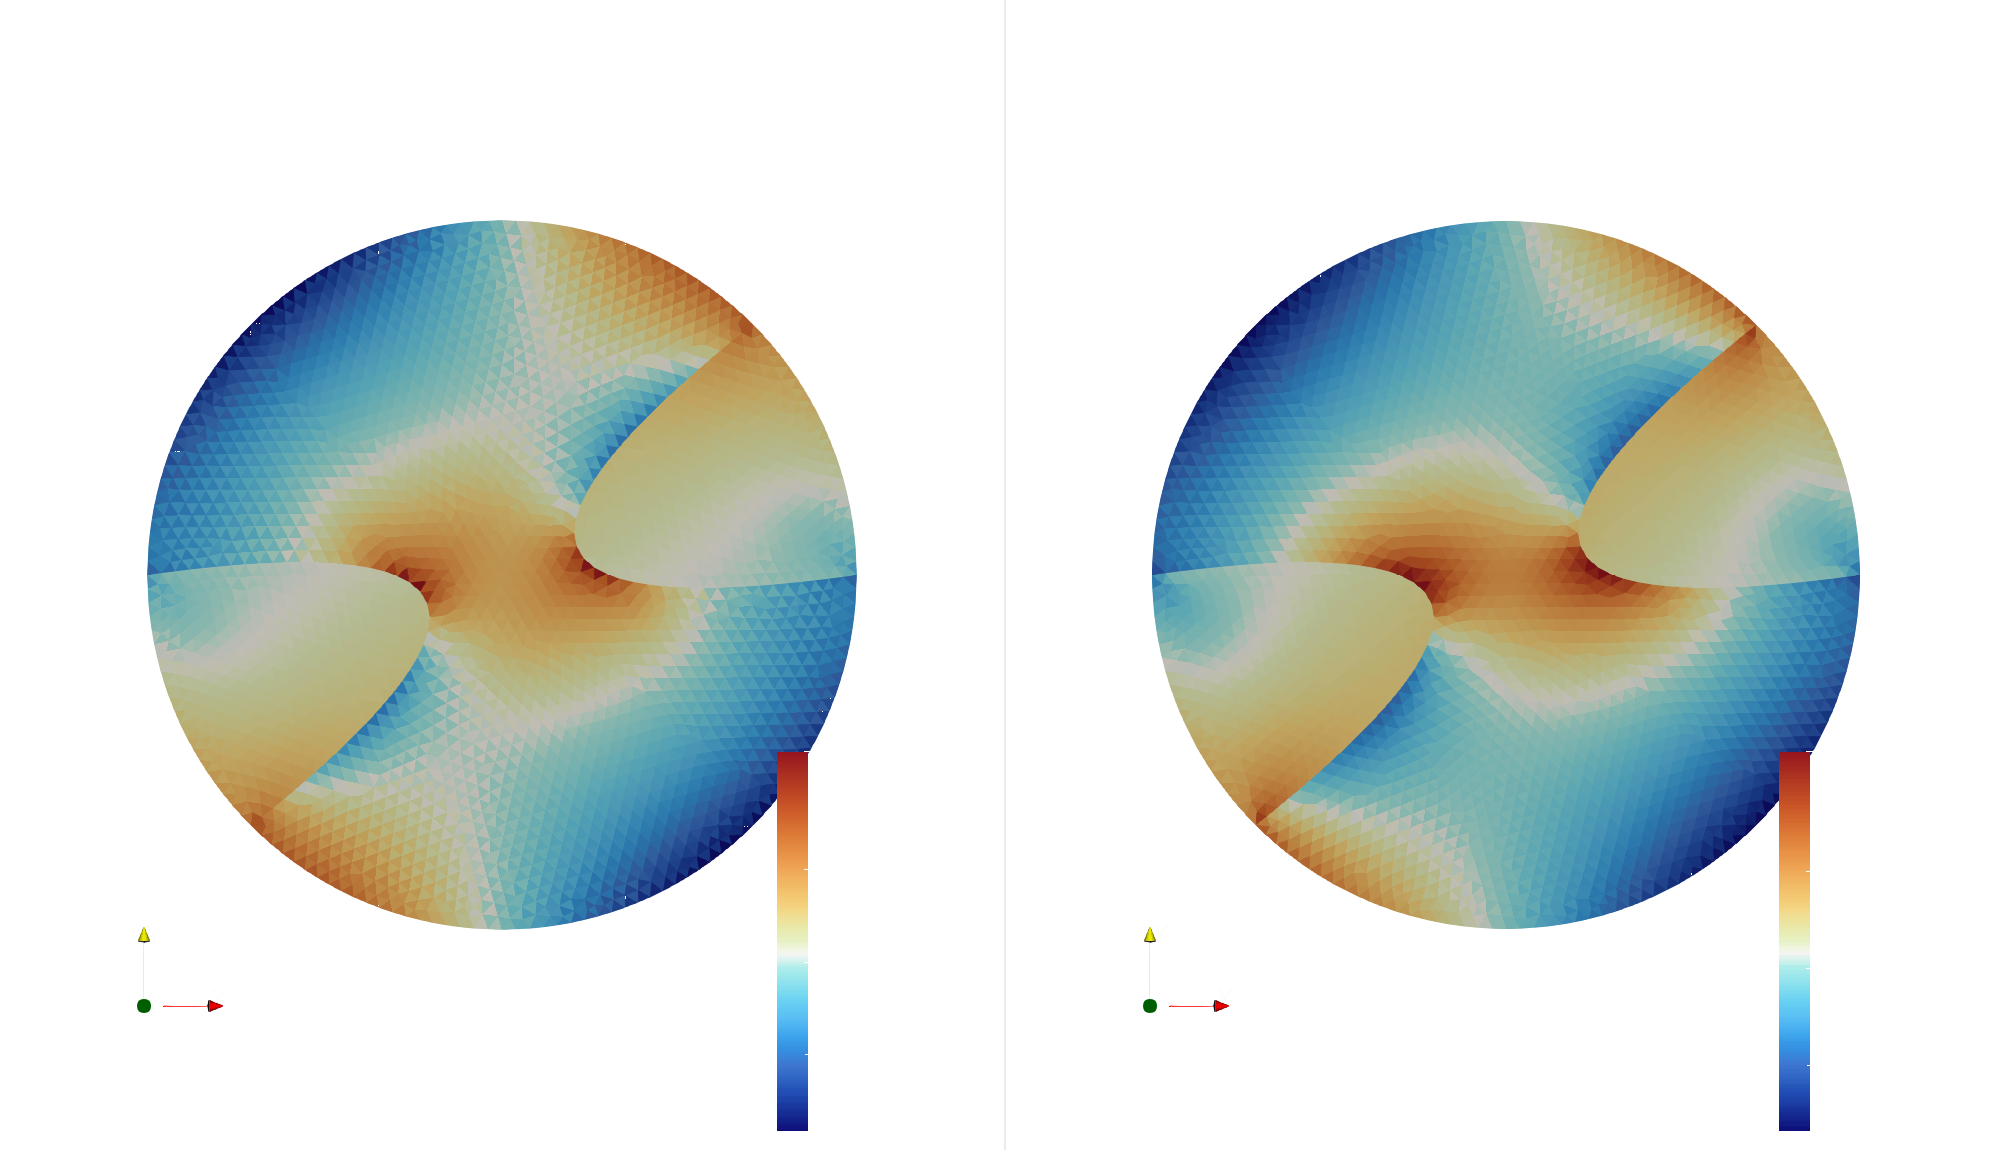
\includegraphics[width=0.8\textwidth]{img/bx_inf_S.png}
\caption{Результаты численного эксперимента: поле напряжений ПК2. Показаны компоненты напряжений $S_{11}$, $S_{22}$ и $S_{12}$, вычисленные моделью CLANN для соответствующих деформаций.}
\label{fig:numerical_stresses}
\end{figure}

\begin{figure}[htbp]
\centering
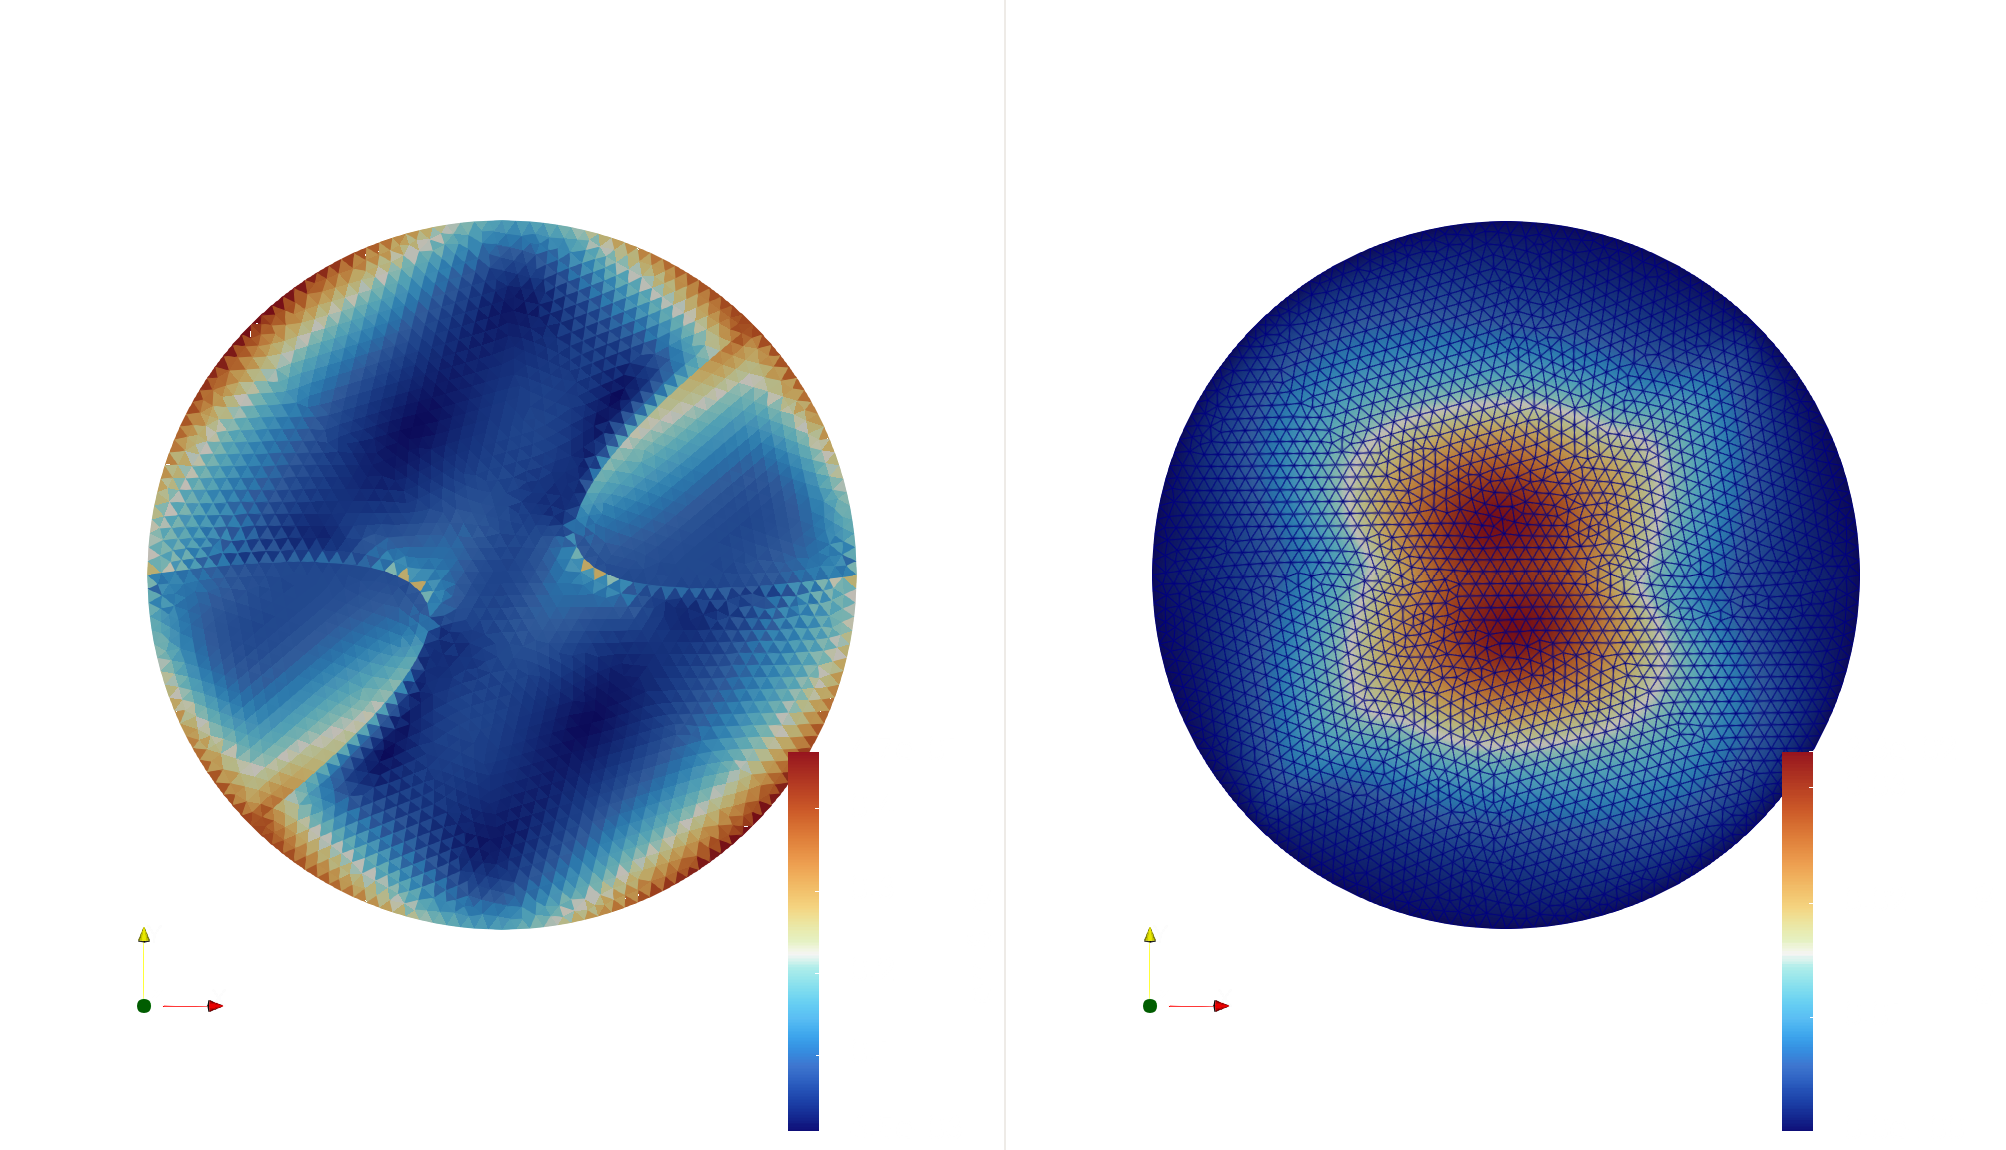
\includegraphics[width=0.8\textwidth]{img/bx_inf_err.png}
\caption{Анализ ошибок численного эксперимента: распределение относительных ошибок между предсказанными и эталонными значениями напряжений. Показаны локальные и глобальные метрики точности модели.}
\label{fig:numerical_errors}
\end{figure}


\section{Натурные эксперименты}
% Здесь будет содержание натурных экспериментов
\subsection{Экспериментальная установка}
% Описание экспериментальной установки

\subsection{Результаты и валидация}
% Результаты натурных экспериментов

\section{Заключение}
% Здесь будет заключение


% \section{Математические и термодинамические свойства}
% \subsection{Выпуклость и устойчивость}
% Строгая выпуклость \(\psi\) обеспечивает единственность минимума, положительную определённость касательной жёсткости и устойчивость численного решения.

% \subsection{Развёрнутый вывод через цепное правило и эквивалентные формы}
% Полная потенциальная энергия деформации задаётся композиционно
% \begin{equation}
%  \Psi(\vect C) = \psi\big(\xi(\vect C)\big),\quad \vect C = \vect F^{\top} \vect F,\quad \vect C = \vect U^{\top} \vect U,\ \xi = (\ln u_{11},\,\ln u_{22},\, u_{12}/u_{11}).
% \end{equation}
% Тензор ПК2 определяется как
% \begin{equation}
%  \vect S = \frac{\partial \Psi}{\partial \vect C}.
% \end{equation}
% Применяя цепное правило к \(\Psi(\vect C)\), получаем эквивалентную запись
% \begin{equation}
%  \frac{\partial \Psi}{\partial \vect C} = \frac{\partial \psi}{\partial \xi} : \frac{\partial \xi}{\partial \vect C} \equiv \vect g(\xi) : \vect J(\vect C),
% \end{equation}
% где \(\vect g(\xi)=\partial\psi/\partial\xi\in\mathbb{R}^3\) и \(\vect J(\vect C)=\partial\xi/\partial \vect C\) — тензор Якоби. В размерности 2D при выбранной параметризации и разложении Холецкого \(\vect C=\vect U^{\top} \vect U\) аналитическая подстановка даёт явные формулы для компонент \(\vect S\).


